\documentclass[12pt]{article} %V1.0
\usepackage{amsfonts,amssymb,amsmath,mathrsfs,amsthm}
\usepackage{graphicx,caption,lipsum}
\usepackage{epsfig,epstopdf}
\usepackage{nccmath}
%\usepackage{harvard}

%\usepackage[margin=2cm]{geometry}
\usepackage[bottom=1in,top=1in,left=1in,right=1in]{geometry}
\setlength{\parindent}{0cm}

%\setlength{\leftmargini}{16pt}

\usepackage[dvipsnames]{xcolor} % en.wikibooks.org/wiki/LaTeX/Colors
\usepackage{enumitem} % bullet points
\usepackage{cmap} % fix the 'fi' problem
\usepackage{rotating,wrapfig,lscape}
\usepackage{bbm}
\usepackage{mathtools} % for multi-lined equations
\usepackage[utf8]{inputenc}
\usepackage[english]{babel}

\usepackage[export]{adjustbox}
\usepackage{setspace}

\onehalfspacing



\newtheorem{theorem}{Theorem}
\newtheorem{corollary}{Corollary}[theorem]
\newtheorem{lemma}[theorem]{Lemma}
\newtheorem{proposition}{Proposition}
 

\linespread{1.25}
\setlength{\parindent}{24pt}



% HYPERLINK
\usepackage[breaklinks=true]{hyperref}
\hypersetup{
  colorlinks=true,
  citecolor=darkblue,
  linkcolor=darkblue,
  urlcolor=darkblue,
  pdfpagemode=none,
  pdfstartview={XYZ null null 1},
  pdftitle={},
  pdfauthor={GH},
  pdfkeywords={} }
\definecolor{darkblue}{rgb}{0,0,0.25}
%

% BIBLIOGRAPHY
\usepackage[longnamesfirst]{natbib}
\bibliographystyle{chicago}
%\bibliographystyle{econometrica}

% DEFINITIONS
\theoremstyle{definition}
\newtheorem{definition}{Definition}%[section]

\captionsetup[figure]{labelsep=period}

\usepackage{palatino}

\setlength{\footnotesep}{1em}

\usepackage{nameref}

\graphicspath{{./figs181014/}}
%---------------------------------------------------------------------------------

\begin{document}

%---------------------------------------------------------------------------------


\noindent {\large \textbf{Extensions}}   

\vspace{0.5cm}

\noindent \normalsize  \textbf{Shisham Adhikari}

\noindent University of California - Davis

\vspace{0.7cm}


\normalsize

\section*{Regain skill in later career}

\begin{figure}[here]
	\centering
	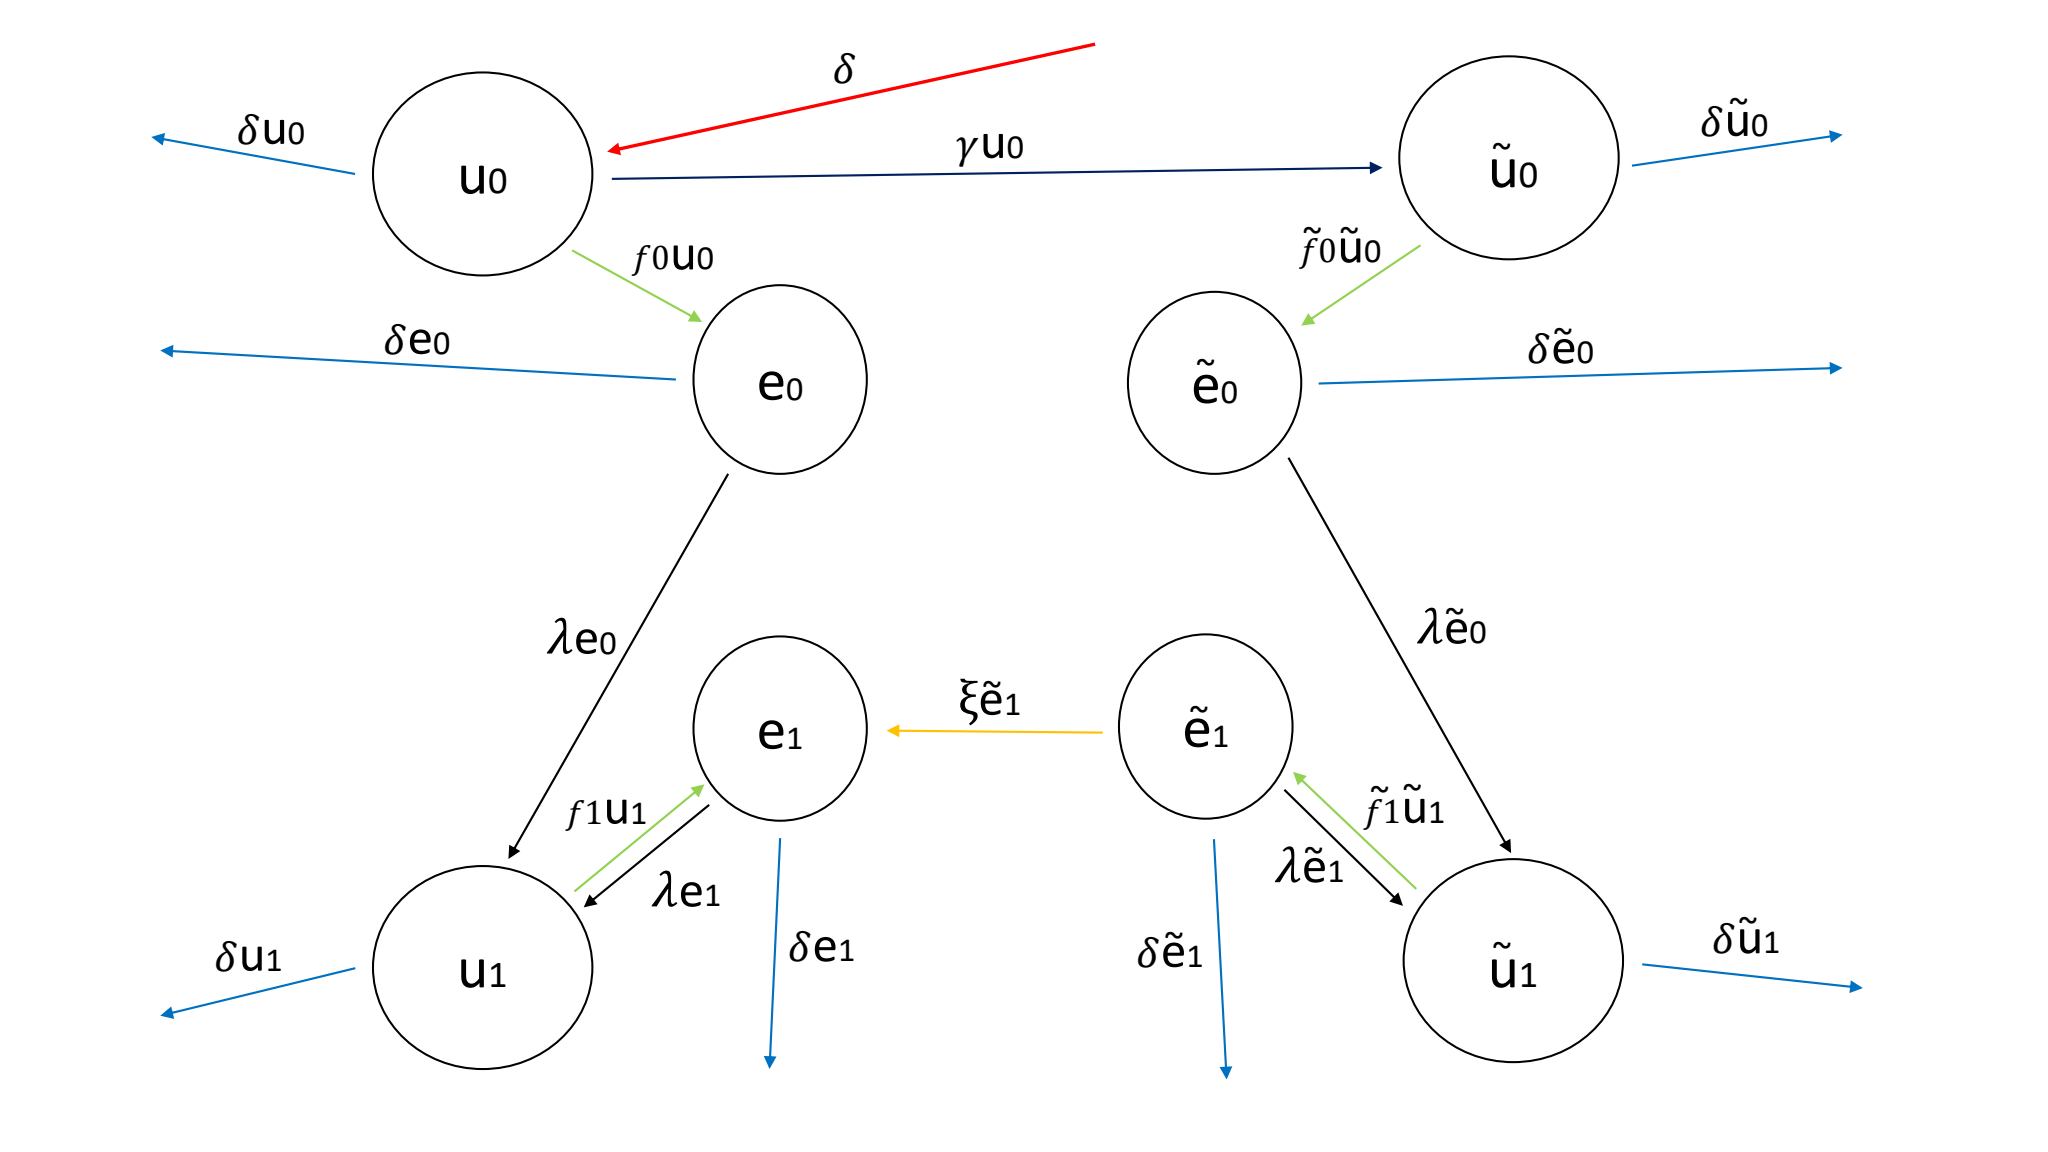
\includegraphics[width=1\linewidth]{figure_E2.png}
 \vspace{-1cm}
	\caption{Worker flows in and out of the various states with regain of skills.}
	\label{figure model}
\end{figure}

\subsection*{Beveridge curves}\label{regain beveridge}
Equating the flows in and out of each state, and after some algebra, we can show that the steady state measure of workers in the various states are as follows:
\begin{eqnarray}
u_0 &=& \frac{\delta}{\delta+\gamma+f_0},  \\
\tilde{u_0} &=& \frac{\gamma}{\delta+\Tilde{f_0}} \cdot  \frac{\delta}{\delta+\gamma+f_0}, \\
e_0 &=& \frac{f_0}{\delta+\lambda} \cdot \frac{\delta}{\delta+\gamma+f_0}, \\
\Tilde{e_0} &=& \frac{\Tilde{f_0}}{\delta+\lambda} \cdot \frac{\gamma}{\delta + \Tilde{f_0}} \cdot \frac{\delta}{\delta+\gamma+f_0},  \\
 \tilde{u_1} &=& \frac{\lambda (\delta+\lambda+\xi) \tilde{f_0} \gamma \delta}{[\delta(\delta+\lambda+\xi)+\tilde{f_1}(\delta+\xi)](\delta+\lambda)(\delta+\tilde{f_0})(\delta+\gamma+f_0)}, \\
  \tilde{e_1} &=& \frac{\tilde{f_1}\lambda \tilde{f_0} \gamma \delta}{[\delta(\delta+\lambda+\xi)+\tilde{f_1}(\delta+\xi)](\delta+\lambda)(\delta+\tilde{f_0})(\delta+\gamma+f_0)},   \\
  u_1 &=& \frac{\lambda}{(\gamma+\delta+f_0)(\delta+\lambda+f_1)}\left[f_0 + \xi \frac{\lambda \gamma \tilde{f_0} \tilde{f_1}}{[\delta(\delta+\lambda+\xi)+\tilde{f_1}(\delta+\xi)](\delta+\lambda)(\delta+\tilde{f_0})} \right],  \\
  e_1 &=& \frac{1}{(\delta+\lambda)(\delta+\lambda+f_1)}\left[\frac{f_0f_1\lambda}{\delta+\gamma+f_0} + \xi \frac{(\delta+\lambda)(\delta+f_1)}{\delta} \tilde{e_1} \right]. 
 \end{eqnarray}

\subsection*{Value Functions}\label{regain value functions}
We move to the steady state value functions, and we start with the firms. Under this extension, the value function of a vacant firm is same as before:
\begin{equation}
   rV = -c + q_0 (J_0-V) + \Tilde{q_0}(\Tilde{J_0}-V) + q_1 (J_1-V) + \Tilde{q_1}(\Tilde{J_1}-V).\nonumber 
\end{equation}Free entry implies that in equilibrium we must have $V=0$, therefore, we can state the free entry condition as 
\begin{equation}
   c= q_0 J_0 + \Tilde{q_0}\Tilde{J_0} + q_1 J_1 + \Tilde{q_1}\Tilde{J_1}.\label{eq free entry} 
\end{equation}

We also have four value functions for productive firms in the various states, i.e., for firms who matched with the four different types of workers (type 0, $\tilde{0}$, 1, and $\tilde{1}$). These are given as follows:   
\begin{eqnarray}
    rJ_0 &=&p-\kappa-w_0-\lambda J_0 - \delta J_0,\label{eq J0} \\
    r\Tilde{J_0} &=&p-\kappa-\Tilde{\kappa}-\Tilde{w_0}-\lambda \Tilde{J_0} - \delta \Tilde{J_0},\label{eq J0 tilde}\\
    rJ_1 &=&p-w_1-\lambda J_1 - \delta J_1, \label{eq J1} \\
        r\Tilde{J_1} &=&p-\Tilde{\kappa}-\Tilde{w_1}-\lambda \Tilde{J_1} - \delta \Tilde{J_1} + \xi(J_1-\tilde{J_1}) . \label{eq J1 tilde}
    \end{eqnarray}

Here, all the functions are same as before except the last equation, 
Next, consider the value functions of workers in the various states. The value functions for unemployed workers in the various states are given by: 
\begin{eqnarray}
    rU_0 &=& z+f_0(W_0-U_0)+\gamma(\Tilde{U_0}-U_0) - \delta U_0, \label{eq U0} \\
    r\Tilde{U_0} &=& z+\Tilde{f_0}(\Tilde{W_0}-\Tilde{U_0})- \delta \Tilde{U_0}, \label{eq U0 tilde}\\
    rU_1 &=& z+f_1(W_1-U_1)- \delta U_1, \label{eq U1}\\
    r\Tilde{U_1} &=& z+\Tilde{f_1}(\Tilde{W_1}-\Tilde{U_1})- \delta \Tilde{U_1}. \label{eq U1 tilde} 
\end{eqnarray}
The value functions for employed workers in the various states are given by: 
\begin{eqnarray}
    rW_0 &=&w_0+\lambda(U_1-W_0)- \delta W_0, \label{eq W0} \\
     r\Tilde{W_0} &=& \Tilde{w_0}+\lambda(\Tilde{U_1}-\Tilde{W_0})- \delta \Tilde{W_0}, \label{eq W0 tilde} \\
     rW_1 &=& w_1+\lambda(U_1-W_1)- \delta W_1, \label{eq W1} \\
     r\Tilde{W_1} &=& \Tilde{w_1}+\lambda(\Tilde{U_1}-\Tilde{W_1})- \delta \Tilde{W_1} + \xi(W_1-\tilde{W_1}). \label{eq W1 tilde}
     \end{eqnarray}
Notice that all equations are the same except the last one. 

Now, we solve for the bargaining problems in the various types of meetings to obtain following wage curves. 

\subsection*{Wage Curves}\label{regain wage curves} 
\textbf{Type $0: (1-\eta)(W_0-U_0) = \eta J_0$}
\begin{equation}\label{eq WC0}
 \begin{split}
         w_0 & = \frac{r+\delta+\gamma +f_0}{r+\delta+\gamma+\eta f_0}\eta (p-\kappa) + \frac{(r+\lambda+\delta)(r+f_1+\delta)(r+\gamma+\delta)}{(r+\delta)(r+\delta+\gamma + \eta f_0)(r+\delta+\lambda+f_1)} (1-\eta) z + \\  
 & + \frac{\gamma \Tilde{f_0}\eta(p-\kappa-\Tilde{\kappa}-\Tilde{w_0})}{(r+\delta)(r+\delta+\gamma + \eta f_0)} - \frac{(1-\eta)\lambda f_1 (r+\gamma+\delta)w_1}{(r+\delta)(r+\delta+\gamma + \eta f_0)(r+\delta+\lambda+f_1)}. 
    \end{split}
\end{equation}

\textbf{Type $\Tilde{0}: (1-\eta)(\Tilde{W_0}-\Tilde{U_0}) = \eta \Tilde{J_0}$}
\begin{equation}
\begin{aligned}
    \Tilde{w_0} = 
    &\frac{1}{r+\delta+\eta \Tilde{f_0}}\Biggl\{ 
        (r+\delta+\Tilde{f_0})\eta(p-\kappa-\Tilde{\kappa}) + (r+\delta)(1-\eta)z \\
    &\quad - \frac{\lambda \eta \Tilde{f_1}}{r+\delta+\lambda+\xi} (p-\Tilde{\kappa}-\Tilde{w_1}) - \xi \frac{\lambda \Tilde{f_1} \eta}{(r+\delta+\lambda)(r+\delta+\lambda+\xi)} (p-w_1)
      \Biggr\}.
\end{aligned}
\end{equation}


\textbf{Type 1: $(1-\eta)(W_1-U_1) = \eta J_1$}
\begin{equation}
 w_1 = \frac{\eta p (r+\lambda+\delta+f_1)+(1-\eta)z(r+\lambda+\delta)}{r+\lambda+\delta + \eta f_1}. \label{eq WC 1}
 \end{equation}
 \textbf{Type $\Tilde{1}: (1-\eta)(\Tilde{W_1}-\Tilde{U_1}) = \eta \Tilde{J_1}$}
\begin{align}
% First line (no number)
\Tilde{w_1} 
&= \Biggl\{ 
    \bigl[(r+\delta)\,(r+\delta+\lambda+\xi+\Tilde{f_1}) + \xi\,\Tilde{f_1}\bigr]\,\eta\,(p-\Tilde{\kappa})
    + (1-\eta)\,z\,(r+\delta)\,(r+\lambda+\delta+\xi)
\nonumber \\[6pt]
% SECOND line: we tag (23) here
&\quad + \xi \,\frac{\Tilde{f_1}(r + \delta + \xi) - f_1(r + \delta + \lambda + \xi)}{r + \delta + \lambda}
         \,\eta\,(p - w_1) \Biggr\}
\tag{25}\label{eq:w1-middle-line} \\[6pt]
% Third line (no number)
&\quad \cdot \frac{1}{
  (r + \delta)\,(r + \delta + \lambda + \xi)
  + \eta\,\Tilde{f_1}\,(r + \delta + \xi)
}.
\nonumber
\end{align}

\newpage
\section*{Gain earlier experience}
\begin{figure}[here]
	\centering
	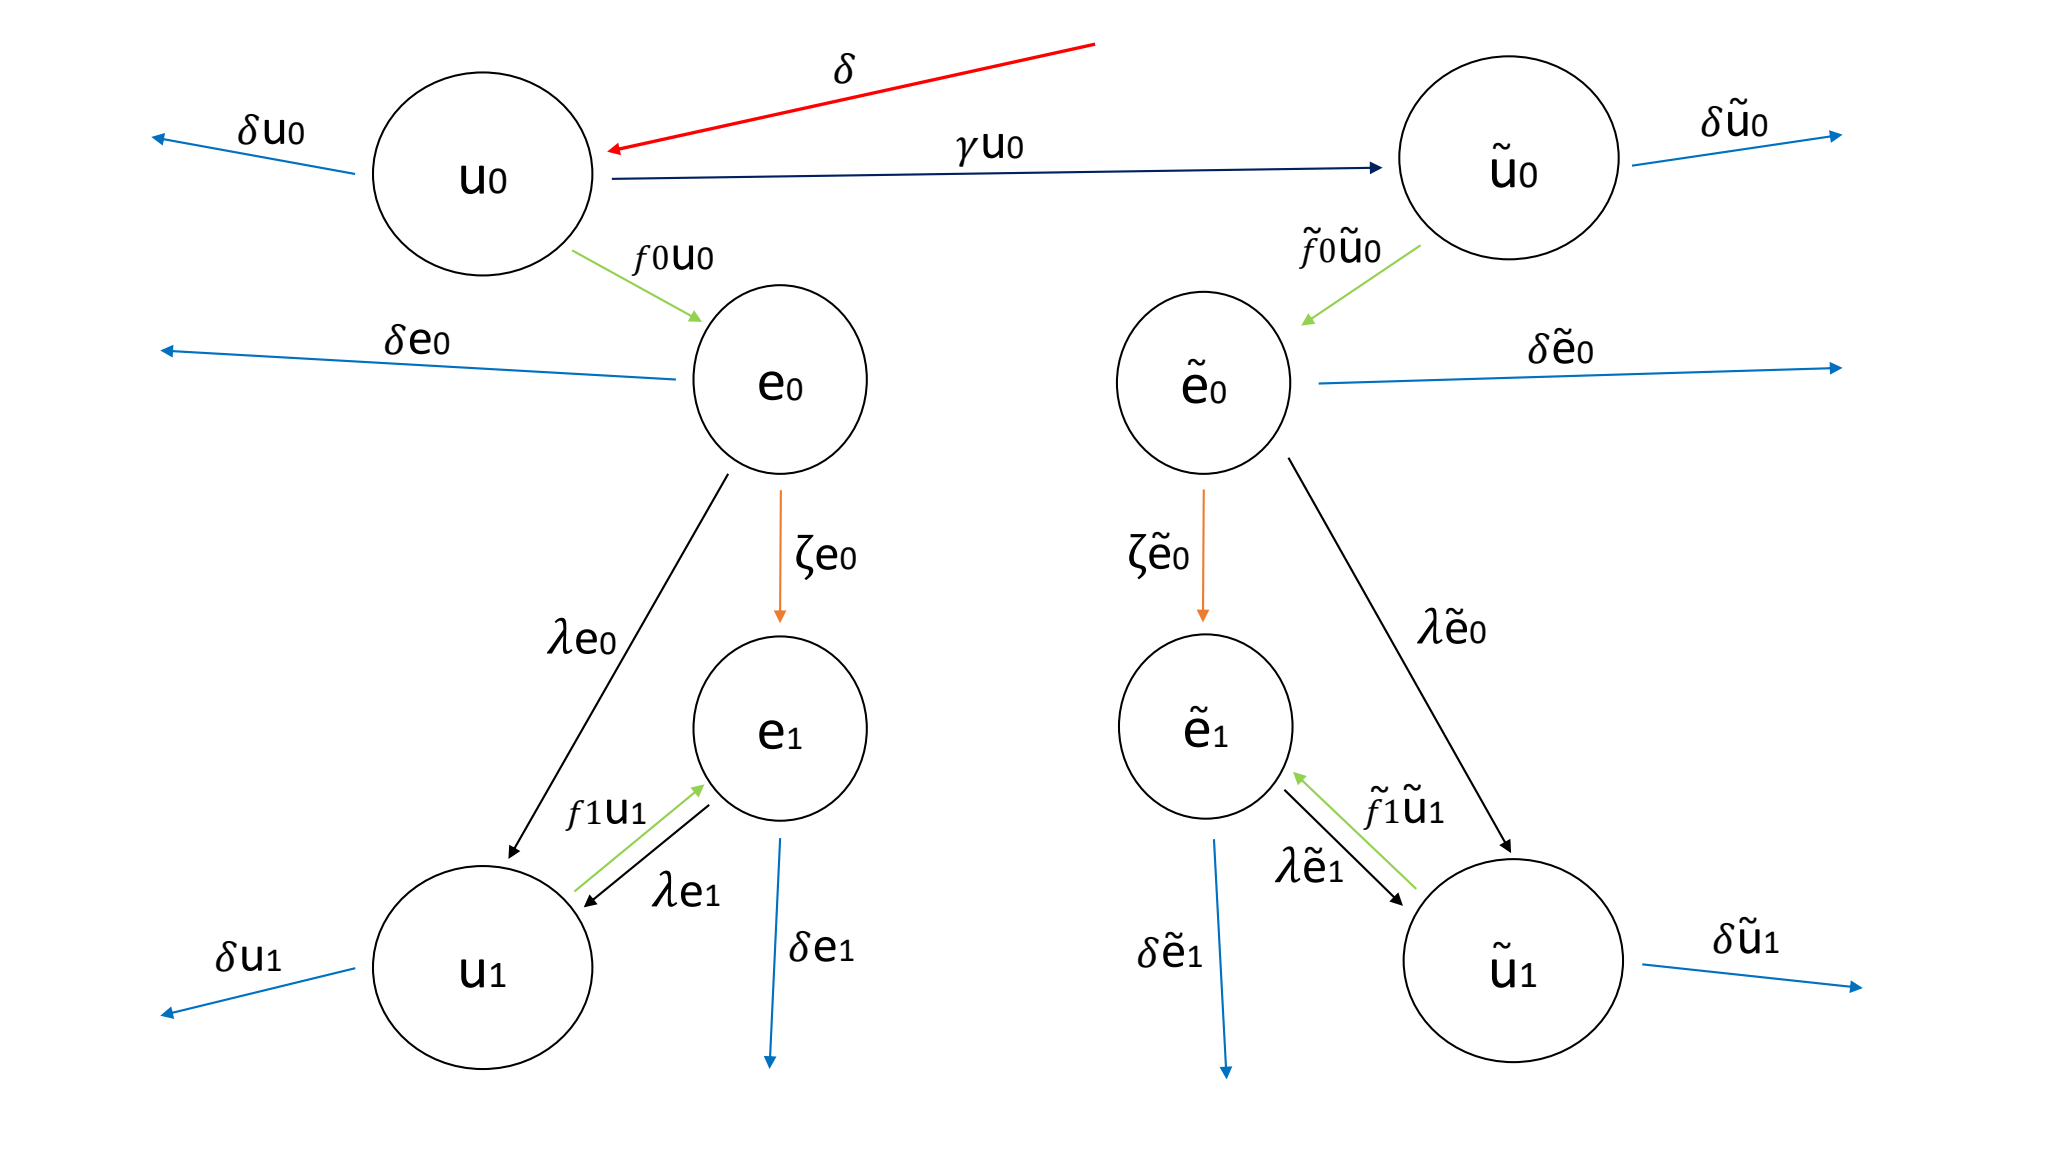
\includegraphics[width=1\linewidth]{figure_E1.png}
 \vspace{-1cm}
	\caption{Worker flows in and out of the various states with regain of skills.}
	\label{figure model}
\end{figure}
\subsection*{Beveridge curves}\label{regain beveridge}
Equating the flows in and out of each state, and after some algebra, we can show that the steady state measure of workers in the various states are as follows:
\begin{eqnarray}
u_0 &=& \frac{\delta}{\delta+\gamma+f_0},  \\
\tilde{u_0} &=& \frac{\gamma}{\delta+\Tilde{f_0}} \cdot  \frac{\delta}{\delta+\gamma+f_0}, \\
e_0 &=& \frac{f_0}{\delta+\lambda} \cdot \frac{\delta}{\delta+\gamma+f_0}, \\
\Tilde{e_0} &=& \frac{\Tilde{f_0}}{\delta+\lambda} \cdot \frac{\gamma}{\delta + \Tilde{f_0}} \cdot \frac{\delta}{\delta+\gamma+f_0},  \\
 \tilde{u_1} &=& \frac{\lambda \Tilde{f_0} \gamma}{(\delta+\lambda+\Tilde{f_1})(\delta+\Tilde{f_0})(\delta+f_0+\gamma)}, \\
  \tilde{e_1} &=& \frac{\Tilde{f_0} \gamma}{(\delta+\lambda)(\delta+f_0+\gamma)(\delta+\Tilde{f_0})} \left[\frac{\lambda \Tilde{f_1}}{\delta+\lambda+\Tilde{f_1}} + \frac{\zeta \delta}{\delta+\lambda+\zeta}\right],   \\
  u_1 &=& \frac{\lambda}{\delta+f_1+\lambda}\frac{f_0}{\delta+f_0+\gamma},  \\
  e_1 &=& \frac{f_0}{(\delta+\lambda)(\delta+f_0+\gamma)}\left[\frac{\lambda f_1}{\delta+\lambda+f_1} +\frac{\zeta \delta}{\delta + \lambda + \zeta} \right]. 
 \end{eqnarray}

\subsection*{Value Functions}
We move to the steady-state value functions, and we start with the firms. Under this extension, the value function of a vacant firm is the same as before:
\begin{equation}
   rV = -c + q_0 (J_0-V) + \Tilde{q_0}(\Tilde{J_0}-V) + q_1 (J_1-V) + \Tilde{q_1}(\Tilde{J_1}-V).\nonumber 
\end{equation}
Free entry implies that in equilibrium we must have $V=0$, therefore, we can state the free entry condition as 
\begin{equation}
   c = q_0 J_0 + \Tilde{q_0}\Tilde{J_0} + q_1 J_1 + \Tilde{q_1}\Tilde{J_1}. 
\end{equation}

We also have four value functions for productive firms in the various states, i.e., for firms who matched with the four different types of workers (type 0, $\tilde{0}$, 1, and $\tilde{1}$). These are given as follows:
\begin{eqnarray}
    rJ_0 &=& p - w_1 - \lambda J_1 - \delta J_1, \\
    r\Tilde{J_1} &=& p - \Tilde{\kappa} - \Tilde{w_1} - \lambda \Tilde{J_1} - \delta \Tilde{J_1}, \\
    rJ_0 &=& p - \kappa - w_0 - \lambda J_0 - \delta J_0 + \zeta (J_1-J_0), \\
    r\Tilde{J_0} &=& p - \kappa - \Tilde{\kappa} - \Tilde{w_0} - \lambda \Tilde{J_0} - \delta \Tilde{J_0} + \zeta (\Tilde{J_1}-\Tilde{J_0}).
\end{eqnarray}

Next, consider the value functions of workers in the various states. The value functions for unemployed workers in the various states are given by:
\begin{eqnarray}
    rU_0 &=& z + f_0 (W_0 - U_0) + \gamma (\Tilde{U_0} - U_0) - \delta U_0, \\
    r\Tilde{U_0} &=& z + \Tilde{f_0} (\Tilde{W_0} - \Tilde{U_0}) - \delta \Tilde{U_0}, \\
    rU_1 &=& z + f_1 (W_1 - U_1) - \delta U_1, \\
    r\Tilde{U_1} &=& z + \Tilde{f_1} (\Tilde{W_1} - \Tilde{U_1}) - \delta \Tilde{U_1}.
\end{eqnarray}

The value functions for employed workers in the various states are given by:
\begin{eqnarray}
    rW_0 &=& w_0 + \lambda (U_1 - W_0) + \zeta(W_1-W_0) - \delta W_0 , \\
    r\Tilde{W_0} &=& \Tilde{w_0} + \lambda (\Tilde{U_1} - \Tilde{W_0}) + \zeta(\Tilde{W_1}-\Tilde{W_0}) - \delta \Tilde{W_0}, \\
    rW_1 &=& w_1 + \lambda (U_1 - W_1)-\delta W_1, \\
    r\Tilde{W_1} &=& \Tilde{w_1} + \lambda (\Tilde{U_1} - \Tilde{W_1}) -\delta \Tilde{W_1}.
\end{eqnarray}
Now, we solve for the bargaining problems in the various types of meetings to obtain the following wage curves.

\subsection*{Wage Curves}\label{regain wage curves} 
\textbf{Type 1: $(1-\eta)(W_1-U_1) = \eta J_1$}
\begin{equation}
 w_1 = \frac{\eta p (r+\lambda+\delta+f_1)+(1-\eta)z(r+\lambda+\delta)}{r+\lambda+\delta + \eta f_1}. \label{eq WC 1}
 \end{equation}
 \textbf{Type $\Tilde{1}: (1-\eta)(\Tilde{W_1}-\Tilde{U_1}) = \eta \Tilde{J_1}$}
\begin{equation}
\Tilde{w_1} = \frac{\eta (p-\Tilde{\kappa}) (r+\lambda+\delta+\Tilde{f_1})+(1-\eta)z(r+\lambda+\delta)}{r+\lambda+\delta + \eta \Tilde{f_1}}. \label{eq WC1 tilde}
\end{equation}
\textbf{Type $\Tilde{0}: (1-\eta)(\Tilde{W_0}-\Tilde{U_0}) = \eta \Tilde{J_0}$}
\begin{equation}
\begin{aligned}
    \Tilde{w_0} = 
    & \frac{1}{r+\delta+\eta \Tilde{f_0}}\left\{ 
        (r+\delta+\Tilde{f_0})\eta(p-\kappa-\Tilde{\kappa}) + (1-\eta)z \left(r+\delta+\frac{(\lambda+\zeta)\Tilde{f_1}}{r+\lambda+\delta+\Tilde{f_1}}\right) \right. \\
    & \quad - \left. \frac{\eta \Tilde{f_0} \zeta (p-\Tilde{\kappa})}{r+\lambda+\delta} - \Tilde{w_1}\left(\frac{\eta \Tilde{f_0} \zeta}{r+\lambda+\delta} + \frac{(1-\eta)(\lambda+\zeta)\Tilde{f_1}}{r+\lambda+\delta+\Tilde{f_1}}\right)
      \right\}.
\end{aligned}
\end{equation}

\textbf{Type $0: (1-\eta)(W_0-U_0) = \eta J_0$}
\begin{equation}
\begin{aligned}
    w_0 = 
    & \frac{1}{r+\delta+\gamma+\eta f_0}\left\{ 
        (r+\delta+\gamma+f_0)\eta(p-\kappa) + \frac{(1-\eta)z}{r+\delta} \frac{[(r+\delta+f_1)(r+\delta+\lambda)+\zeta f_1](r+\delta + \gamma)}{\gamma+\lambda+\delta+f_1}  \right. \\
    & \quad + \left. \eta f_0 \zeta \frac{p-w_1}{r+\delta+\lambda} + \frac{\eta \Tilde{f_0} \gamma}{r+\delta} (p-\kappa-\Tilde{\kappa}-\Tilde{w_0}) \right. \\
    & \quad + \left. \frac{\gamma \Tilde{f_0} \eta}{r+\delta} \zeta (p-\Tilde{\kappa} - \Tilde{w_1}) - \frac{(1-\eta)(\lambda+\zeta)(r+\delta+\gamma)}{r+\delta} f_1 \frac{w_1}{r+\lambda+\delta+f_1}
      \right\}.
\end{aligned}
\end{equation}
\end{document}
